\section{POLICY STABILITY}
% Optimal agents consider the overall effect of a policy, not act greedily with respect to the individual actions. Therefore, in order for the autoregressive policy derived from control-as-inference to be optimal, it has to be stable under making future decisions based on the predictor alone.

In search of the sufficient conditions for the autoregressive goal-conditioned policy to be optimal, one point of focus might be the question of how to \emph{extend} trajectories: we might hope to stitch the optimal trajectory from actions that are optimal at a k-step-lookahead; optimal policies should then be those that behave consistently, in the sense that it would make the same decisions as if it were allowed to take actions looking $k$ steps into the future. Formally, we have the following definition.

\begin{definition}[Policy-stable reasoning]
    Given deterministic dynamics $\tau$ and a prior $p(a_t|s_t)$, we say that a policy $\pi(a_t|s_t) \propto p(\OO_{t:T}|s_t, a_t)$ is \emph{(1-)policy-stable}, if for any actions $a^1_t, a^1_{t+1}, a^2_t, a^2_{t+1}$, with $a^i_{t+1} = \arg\max_{a^i_{t+1}} p(\OO_{t:T}|a^1_{t, t+1}, s_t)$ (where $s^i_{t+1} = \tau(s_t, a^i_t)$), we have that:
    \[
        % \pi(a^1_{t, t+1}|s_t) \geq \pi(a^2_{t, t+1}|s_t) \implies  
        % \pi(a^1_{t}|s_t) \geq \pi(a^2_{t}| s_t)
        p(\OO_{t:T}|a^1_{t, t+1}, s_t) > p(\OO_{t:T}|a^2_{t, t+1}, s_t) \implies  
        p(\OO_{t:T}|a^1_{t}, s_t) > p(\OO_{t:T}|a^2_{t}, s_t)
    \]
    In other words: given that that $a^i_{t+1}$  best continues $a^i_t$, if $(a^1_t, a^1_{t+1})$ is preferred to $(a^2_t, a^2_{t+1})$, then $a^1_t$ should be preferred to $a^2_t$.
    % \[
    %     p(a^1_t, a^1_{t+1}|s_t) \geq \pi(a^2_t, a^2_{t+1}|s_t) \implies  \pi(a^1_t|s_t) \geq \pi(a^1_t|s_t)
    % \]

\end{definition}

\begin{figure}
\centering
% \begin{wrapfigure}{r}{1\textwidth}
    % \vspace{-5mm}
    % \resizebox{1\textwidth}{!}{
    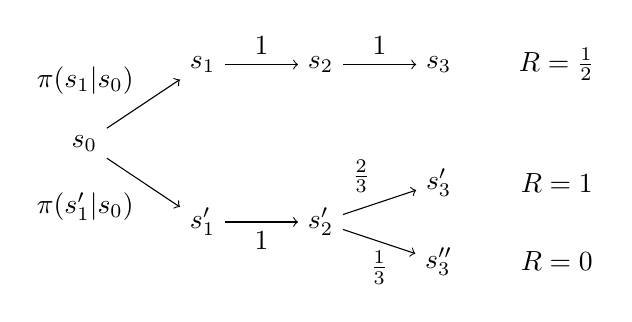
\begin{tikzpicture}
      \node (root) at (0,0) {$s_0$};
      \node (R) at (1.5,1) {$s_1$};
      \node (Rc) at (1.5,-1) {$s'_1$};
      
      \node (RR) at (3,1) {$s_2$};
      \node (RRc) at (3,-1) {$s'_2$};
      
      \node (RcR) at (4.5,1) {$s_3$};
      \node (RcRc) at (4.5,-0.5) {$s'_3$};
      \node (RcRcRc) at (4.5,-1.5) {$s''_3$};
    
      \draw[->] (root) -- (R) node [midway, above left] {$\pi(s_1|s_0)$}; % 
      \draw[->] (root) -- (Rc) node [midway, below left] {$\pi(s'_1|s_0)$}; % 
      
      \draw[->] (R) -- (RR) node [midway, above ] {$1$};
      \draw[->] (Rc) -- (RRc) node [midway, below ] {$1$};
      \draw[->] (RR) -- (RcR) node [midway, above ] {$1$};
      \draw[->] (RRc) -- (RcRc) node [midway, above left] {$\frac{2}{3}$};
      \draw[->] (RRc) -- (RcRcRc) node [midway, below] {$\frac{1}{3}$};
    
      \node at (6,1) {$\Prob{R} = \frac{1}{2}$};
      \node at (6,-0.5) {$\Prob{R} = 1$};
      \node at (6,-1.5) {$\Prob{R} = 0$};
    \end{tikzpicture}
    % }
    \caption{$\pi$ cannot satisfy both 2-policy-stability and 1-policy-stability.}
    \label{fig:not-policy-stable}
    % \vspace{-6mm}
% \end{wrapfigure}
\end{figure}

Unfortunately, not only this is not a sufficient condition - in some instances, it is even contradicting optimality. This is because it is impossible to properly extend the the policy-stability over an arbitrary number of actions. To show that, we can introduce a notion of $n$-policy-stable predictor, which says that for any sequences $a_{1:k}, a'_{1:k}$ and actions $a, a'$, such that the sequence $a_{1:k}$ best continues $a$ and sequence $a'_{1:k}$ best continues $a'$, we have that $(a, a_{1:k})$ being preferred over $(a', a'_{1:k})$ implies that $a$ is preferred to $a'$. 

From direct calculation, it can be seen that, if a policy derived by control-as-inference from a prior over the MDP shown in the \Cref{fig:not-policy-stable} is to be 1-policy-stable, then it must be the case that $\pi(s_1|s_0) \geq \pi(s'_1|s_0)$, while considering two actions into the future and then following the prior, moving into $s_2$ is a better choice. However, to be 2-policy-stable, it has to satisfy $\pi(s_1|s_0) < \pi(s'_1|s_0)$, since after considering three moves in the future, moving to $s'_1$ becomes the better choice. Since 1-policy-stable and 2-policy-stable are mutually exclusive for a policy derived by control-as-inference from this prior, one has to make a choice as to which $n$-policy-stability to require, which, in practice, requires the knowledge of the time horizon (and for it to be fixed and finite).
